% !TeX spellcheck = es_ES
\chapter{Propuesta}\label{chapter:proposal}


%- Explicar un poco cómo se le da solución a los problemas detectados en el capítulo anterior, para describir un poco de forma general las características del método propuesto.
%
%- Realizar una introducción sobre el contenido y la estructura del capítulo

En este capítulo se presenta un método para la selección de ``flujos de algoritmos'' usando técnicas de meta-learning. Un flujo puede ser visto como un caso especial de algoritmo que aplica cada algoritmo de forma secuencial a la salida del algoritmo anterior en la sucesión. Por lo tanto, como un flujo está compuesto de varios algoritmos, la búsqueda de estos y de sus hiperparámetros resulta más compleja. 

La herramienta de meta-learning creada es capaz de abordar una gran variedad de problemas mediante la selección de meta-características capaces de representarlos. Además, explorando la interacción entre las características de los datasets y la estructura de los flujos, el método propuesto es capaz de identificar flujos con un buen rendimiento sin realizar un análisis computacionalmente costoso. Como sistema de AutoML complementario se eligió AutoGOAL, que destaca por la gran cantidad de técnicas y herramientas que utiliza, permitiéndole resolver una amplia gama de tareas. AutoGOAL es utilizado para la generación de flujos de algoritmos para crear la base de conocimiento, por lo que, debido a la variedad de herramientas de ML que AutoGOAL utiliza, se presenta gran diversidad en los flujos guardados.


El enfoque desarrollado se propone como un paso preliminar para otras soluciones más costosas computacionalmente, como por ejemplo, para la inicialización de sistemas de AutoML. En esta investigación AutoGOAL también es utilizado como herramienta complementaria en el proceso de búsqueda de flujos. Por lo tanto, se describe como se realiza la adición de conocimiento experto a la estrategia de búsqueda utilizada por AutoGOAL: Evolución Probabilística Gramatical (\textit{Probabilistic Grammatical Evolution})~\cite{pge2015}, que no había sido utilizada anteriormente con meta-learning.


Este capítulo proporciona una descripción al método de meta-learning propuesto para la selección de flujos (Sección~\ref{sec:proposal}) y un ejemplo de su incorporación a un sistema de AutoML (Sección~\ref{sec:autogoal_imp}). La propuesta es descrita explicando cómo ocurre la adquisición de meta-conocimiento (Sección \ref{sub:adquisicion}), que permite la creación de una base de conocimiento, mostrando las meta-características utilizadas y cómo los flujos de algoritmos fueron generados y guardados. Luego, se describe cómo se aplica el meta-conocimiento (Sección \ref{sub:aplicacion}), mediante la implementación de dos estrategias que tienen el objetivo de recomendar una lista de flujos de algoritmos prometedores para un dataset determinado. Por último, se explica cómo esta lista de flujos resultantes generada por el método propuesto es añadida al proceso de búsqueda de AutoGOAL (Sección~\ref{sec:autogoal_imp}).

\section{Método propuesto}\label{sec:proposal}

%- Un sistema meta-learning está compuesto por dos fases: la fase offline, que es de aprendizaje, en donde ocurre la adquisición de meta-conocimiento y la fase online, que es de recomendación, en donde se aplica el meta-conocimiento, explicar el proceso de meta-learning explicando cada una de estas fases.
%+ Poner una gráfica para explicar mejor cómo se realizan estos procesos.
%
%- Hablar de la estructura de esta sección, que se separa en dos partes para profundizar cómo se realiza la adquisición y aplicación del meta-conocimiento.

El enfoque de meta-learning propuesto está compuesto por dos fases:
\begin{itemize}
	\item La fase offline, que es de aprendizaje, es donde ocurre la adquisición de meta-conocimiento. El objetivo de esta parte es obtener los meta-datos necesarios para la solución del problema de meta-learning propuesto: la obtención de un ranking de flujos de algoritmos de aprendizaje para una determinada tarea. En esta fase se obtiene una caracterización de los datasets y el rendimiento de un conjunto flujos de algoritmos en dichos datasets.
	\item La fase online, que es de recomendación, es donde se aplica el meta-conocimiento adquirido en la fase anterior. En esta fase, dada una tarea con los meta-datos ganados del análisis de las tareas similares y el entrenamiento de flujos de algoritmos en dichos datasets, el objetivo es producir una lista de los flujos prometedores para resolver la tarea inicial.
\end{itemize}

La Figura~\ref{fig:system} muestra el flujo de trabajo de la estrategia de meta-learning implementada. En la fase offline (Figura~\ref{fig:system} derecha) se obtiene una caracterización de los datasets y la estructura y rendimiento de un conjunto flujos de algoritmos en dichos datasets, esta información es utilizada para entrenar el meta-modelo. En la fase online (Figura~\ref{fig:system} izquierda), dado un nuevo dataset, se extraen sus meta-características y de acuerdo a estas se seleccionan los datasets similares. De estos datasets se obtienen los flujos de algoritmos guardados en la base de conocimiento y con estos y el meta-modelo se genera un ranking final de flujos de algoritmos.


\begin{figure}[H]
	\centering
	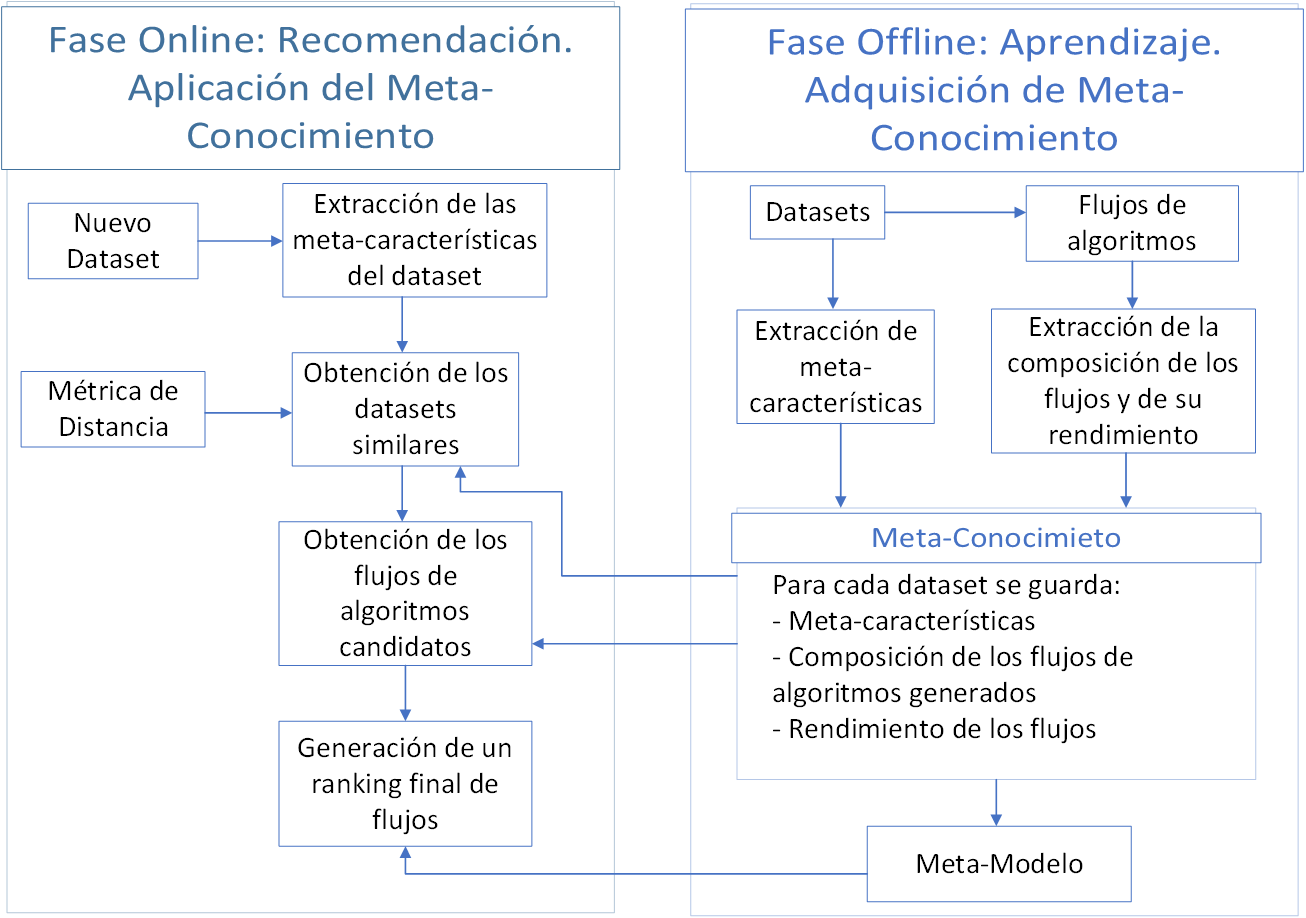
\includegraphics[scale=.4]{Figures/system.png}
	%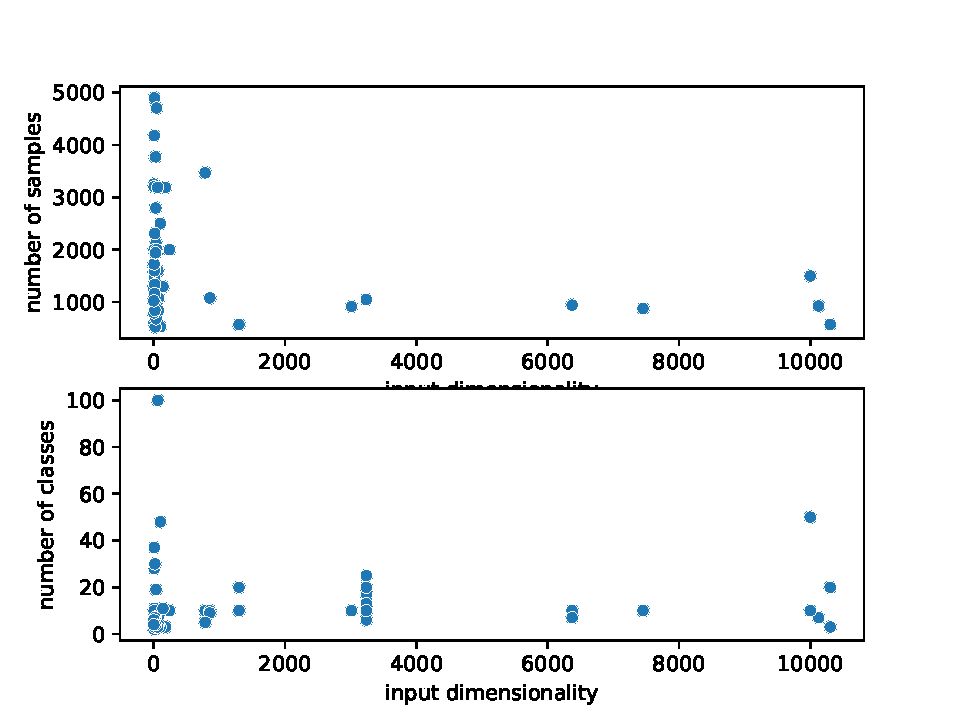
\includegraphics[scale=.60]{Figures/mtf scatterplot.pdf}
	\caption{Flujo de trabajo del enfoque de meta-learning propuesto.}
	\label{fig:system}
\end{figure}

La implementación de cada uno de estas fases es descrita en las siguientes secciones con más profundidad.

\subsection{Adquisición de meta-conocimiento}\label{sub:adquisicion}

%- Explicar cómo se realiza la adquisición de meta-conocimiento, con la extracción de meta-features y de información sobre los pipelines usados.
%- Explicar la importancia de las meta-features. Las meta-features extraídos de cada dataset deben ser suficientes para describir los aspectos principales del dataset, de tal manera que cada dataset pueda ser identificado mediante esta caracterización. Además, deben comprender las características necesarias para distinguir el rendimiento obtenido de diferentes algoritmos de aprendizaje cuando son aplicados a este dataset. 
%- Recordar un poco los distintos tipos de meta-features, describiéndolos un poco: simples, generales, estadísticas, teóricas de la información, basados en modelos, _landmarking_. Explicar que estos últimos dos no fueron implementados debido a su complejidad computacional.
%- Explicar la información que se extrajo sobre los pipelines: para cada dataset se extrajeron los mejores pipelines, explicar el formato en que fueron guardados (mediante el sampler de AutoGOAL), y el rendimiento que se obtuvo para cada uno de ellos.
%- Concluir mencionando que las meta-features y la estructura de los pipelines son usadas como características para el meta-modelo, y el rendimiento de los pipelines como etiquetas.

La adquisición de meta-conocimiento se realiza mediante la extracción de caracterizaciones de un conjunto de datasets, es decir, meta-características, y de información referente a un conjuntos de algoritmos que deben ser probados en estos datasets. Entre los datos de los algoritmos extraídos se guarda información respecto a los hiperparámetros utilizados y al rendimiento alcanzado en cada una de las tareas para cada uno de los conjuntos de algoritmos usados.

\subsubsection{Características de los datasets}\label{subsub:metafeat}

Para extraer meta-características de una tarea de aprendizaje específica es necesario realizar un análisis de la información contenida en el dataset asociado a ella. Las meta-características, además de proveer información referente a los datos del dataset (relacionados a valores medios, desviación estándar, etc), deben ser capaces de proporcionar conocimiento sobre la tarea que el dataset está representando.  Por lo tanto, las meta-características pueden ser concebidas como colecciones específicas de características de un dataset, las cuales proporcionan información relevante sobre la tarea que es necesario resolver mediante algoritmos de aprendizaje~\cite{castiello2005metadata}. La principal suposición es que el conocimiento codificado en las meta-características deben mostrar algún tipo de pista general (por ejemplo, relacionado a la complejidad de la tarea) que permita la solución de la tarea, en vez de limitarse a la información relacionada con el contenido del dataset (como la composición de sus datos). Con estas meta-características y una cantidad suficientemente grande de datasets es posible la creación de un meta-modelo que sea capaz de resolver una gran cantidad de tareas.

% Las meta-features extraídos de cada dataset deben ser suficientes para describir los aspectos principales del mismo, de tal manera que cada dataset pueda ser identificado mediante esta caracterización. Además, deben comprender las características necesarias para distinguir el rendimiento obtenido de diferentes algoritmos de aprendizaje cuando son aplicados. 

Como se mencionó anteriormente en el Capítulo \ref{chapter:review}, las meta-características se pueden separar en 5 categorías \cite{bradzil2009metalearning}:

\begin{itemize}
	\item \textit{Simples o generales:} Incluyen información general relacionada a un dataset determinado y, en cierta medida, están concebidas para medir la complejidad del problema subyacente.
	\item \textit{Estadísticas:} Describen las propiedades numéricas de una distribución de datos. Pueden ser empleadas para tener en cuenta el número de propiedades, lo que le permite al meta-modelo discriminar el grado de correlación de los atributos numéricos y estimar su distribución.
	\item \textit{Teóricas de la información:} Son características del campo de teoría de la información, apropiadas particularmente para describir atributos categóricos, pero también pueden ajustar atributos continuos. Semánticamente, describen la variedad y la redundancia de los atributos utilizados para representar las clases.
	\item \textit{Basados en modelos:} están caracterizadas por la extracción de información de un modelo de aprendizaje de predicción, generalmente, un árbol de decisión.
	\item \textit{Landmarking:} Usan el rendimiento de algoritmos de aprendizaje simples y rápidos para caracterizar los datasets.
\end{itemize}

Debido a la complejidad computacional requerida para el cálculo de los últimos dos tipos de meta-características, estos no fueron implementados. Sin embargo, se añadieron meta-características específicas de AutoGOAL, aprovechando la caracterización de los tipos semánticos de entrada y de salida que este sistema ofrece. Para evaluar el enfoque seguido se implementaron las siguientes meta-características, tomadas varios trabajos del estado del arte \cite{castiello2005metadata, fuerer2015efficient}.

\begin{itemize}
	\item \underline{\textsc{Simples}}: \begin{description}
		\item[Es supervisado:] determina si un problema es supervisado o no.
		\item[Tamaño de la muestra:] representa el número total \texttt{k} de instancias en el dataset (la cardinalidad del dataset).
		\item[Número de clases:] representa la cantidad de posibles de clases (etiquetas) presentes en el dataset que son posibles predecir.
		\item[Dimensionalidad de la entrada:] representa el número total de \texttt{m} atributos en el dataset.
		\item[Dimensionalidad de la salida:] representa el número total de valores de salida en el dataset.
		\item[Dimensionalidad del dataset:] representa la proporción entre el número de atributos y el número de observaciones del dataset, es decir, $dim_{data} = \dfrac{m}{k}$.
		\item[Cantidad de características categóricas:] cantidad de atributos del dataset que tienen valores categóricos.
		\item[Características categóricas:] determina si el dataset tiene atributos que tienen valores categóricos.
		\item[Cantidad de características numéricas:] cantidad de atributos del dataset que tienen valores numéricos.
		\item[Características numéricas:] determina si el dataset tiene atributos que tienen valores numéricos
		\item[Cantidad de valores faltantes]
	\end{description}
	\item \underline{\textsc{Estadísticos}}: \begin{description}
		\item[Desviación estándar:] estima la dispersión de la variable aleatoria $X = x_1, x_2, ..., x_k$ (las características del dataset) con respecto a su media $\overline{X} = \dfrac{1}{k}\sum^k_{i=1}x_i$. Es calculada como $std_X = \sqrt{\dfrac{1}{k}\sum^k_{i=1}xi - \overline{X}}$
		\item[Coeficiente de variación:] evalúa la normalización de la desviación estándar de la variable aleatoria X con respecto a su valor medio: $VarCoeff_X =  \dfrac{std_x}{\overline{X}}$
		\item[Covarianza media:] la covarianza expresa la relación lineal entre dos variables aleatorias $X = x_1, ..., x_k$ y $Y = y_1, ..., y_k$ y está definida como: $Cov(X, Y) = \sum^k_{i=1} \dfrac{(x_k - \overline(X))(y_k - \overline{Y})}{k-1}$. La media de la covarianza entre todos los pares de atributos se usa como medida de covarianza de todo el dataset.
		\item[Coeficiente de correlación lineal:] análisis de correlación que intenta medir la fuerza de una relación entre dos variables aleatorias $X$ y $Y$. Puede ser estimado usando la siguiente fórmula: $\rho_{X, Y} = \dfrac{Cov(X, Y}{\sqrt{std_X std_Y}}$. Como coeficiente de correlación lineal de todo el dataset se usa el promedio de las correlaciones entre todos los pares de atributos.
		\item[\textit{Skewness} (Oblicuidad):] mide la falta de simetría en la distribución de una variable aleatoria X, en este caso todo el dataset, para cada uno de los atributos. El resultado es un \texttt{array}, que es caracterizado devolviendo el valor medio, máximo, mínimo y la desviación estándar.
		\item[Curtosis:] mide el grado de concentración que presentan los valores de una variable alrededor de la zona central de la distribución de frecuencias, en este caso todo el dataset. El resultado es un \texttt{array}, que es caracterizado devolviendo el valor medio, máximo, mínimo y la desviación estándar.
		\item[PCA (\textit{Principal Component Analysis}, Análisis de los Componentes Principales):] es un método para transformar un determinado dataset en un nuevo dataset de dimensiones reducidas, para concentrar la información sobre las diferencias entre las instancias en un pequeño número de dimensiones. En el contexto de PCA, el primer componente es un vector que representa la dirección de máxima varianza. Por estas razones se realiza el análisis de los componentes principales, y se retorna el \textit{skewnes} y la curtosis del primer vector.
	\end{description}
	\item \underline{\textsc{Teóricos de la Información}}: \begin{description}
		\item[Entropía normalizada de una clase:]  el valor de entropía $H(C)$ de una variable $C$ indica cuanta información es necesaria para especificar una clase (etiqueta). El valor de entropía $H(C)$ es evaluado usando la siguiente fórmula: $H(C) = \sum^n_{i=1}p_i log_2(p_i)$, donde $p_i$ es la probabilidad (frecuencia relativa) de ocurrencia de una clase $i$. Cuando suponemos que cada clase en un dataset tiene la misma probabilidad de aparecer, entonces el valor máximo teórico para la entropía de una clase es $log_2(n)$, por lo tanto la entropía normalizada es calculada como: $H(C)_{norm} = \dfrac{H(C)}{log_2(n)}$
		\item[Entropía normalizada de un atributo:] el valor de entropía H(X) de un atributo X mide la información relacionada a los valores que X puede tener. La entropía normalizada de un atributo se calcula con la misma fórmula anterior: $H(X)_{norm} = \dfrac{H(X)}{log_2(n)}$. Para retornar un valor representado la entropía de todo el dataset se calcula la entropía de cada uno de sus atributos, y de estos valores es devuelto la media, el mínimo, el máximo y la desviación estándar.
		\item[Entropía conjunta:] mide la entropía total del sistema combinado de variables, es decir, de un par de variables (C, X), los cuales están representados por una variable de clase y uno de los M atributos de entrada discretizados respectivamente. Si $p_{ij}$ representa la probabilidad conjunta de observar el i-ésimo valor del atributo X y el j-ésimo valor de clase, la entropía conjunta está definida como: $H(C, X) = \sum_{i \in X, j \in C} p_{ij} log_2(p_{ij})$. Después de calcular la entropía para cada par clase-atributo, de estos valores se devuelve la media, el mínimo, el máximo y la desviación estándar.
		\item[Información mutua de clase y atributo:] mide la información común compartida entre dos variables aleatorias C y X. Si C y X representan una variable de clase y un atributo de entrada respectivamente, entonces esta meta-característica mide la información contenida por el atributo X sobre una variable de clase y describe la reducción de incertidumbre para C debido al conocimiento de X. La información mutua de clase y atributo es evaluada usando la fórmula: $MI(C, X) = H(C) + H(X) - H(C, X)$. Como medida para describir todo el dataset, se calcula la entropía para cada par clase-atributo, de estos valores se devuelve la media, el mínimo, el máximo y la desviación estándar.
		\item[Número equivalente de atributos:] en lo referente a las tareas de clasificación, la información requerida para especificar una clase es $H(C)$ y ningún sistema de clasificación puede ser completamente existoso a no ser que se proporcione  $H(C)$ pedazos de información. Esta meta-característica proporciona información sobre la complejidad de un problema, específicamente el número de atributos de un dataset determinado que es adecuado para resolver la tarea de clasificación. Es evaluada mediante la proporción entre la entropía de clase $H(C)$ y el promedio de la información mutua $\overline{MI(C, X)}$ como: $EN_{attr} = \dfrac{H(C)}{\overline{MI(C, X}}$
		\item[Relación de la señal de ruido:]  mide la cantidad de información irrelevante contenida en un dataset. Si se considera $\overline{MI(C, X)}$ como una medida de información útil de una clase y $\overline{H(X)} - \overline{MI(C, X)}$ como una medida de información no útil, la meta-característica puede ser evaluado como: $NS.ratio = \dfrac{\overline{H(X)} - \overline{MI(C, X}}{\overline{MI(C, X)}}$
	\end{description}
	\item \textsc{\underline{Específicos de AutoGOAL}}: \begin{description}
		\item[Tipo semántico de la entrada y de la salida:] AutoGOAL representa diferentes tipos de datos semánticos que recogen el concepto de compatibilidad de tipos. Estos tipos se representan como una jerarquía de clases en la cual la herencia determina la relación de compatibilidad $\leq$. Los tipos de datos tienen una interpretación semántica más allá de su estructura computacional subyacente. Por ejemplo, una lista de valores puede representar un vector de valores discretos o un vector de categorías, dependiendo de la interpretación más adecuada para un problema determinado. En su implementación actual, AutoGOAL define 23 tipos semánticos de datos, incluyendo varios para datos de lenguaje natural, como \texttt{Token} o \texttt{Stem}.
	\end{description}
\end{itemize}

Es posible la caracterización de estas meta-características por más de un aspecto, además de la categorización por tipos estudiada. Por ejemplo, el tipo de tarea de ML que describe. Algunas meta-características están restringidas a tareas específicas, como la clasificación, mientras otras pueden aplicarse de manera más genérica a tareas supervisadas, como problemas de regresión. En las tareas supervisadas y de clasificación, se requiere un atributo de destino para evaluar las meta-características, que no es necesario para las meta-características de cualquier tipo. Las meta-características clasificadas como ``Cualquiera'' son las más generales y también se pueden aplicar a tareas no supervisadas como clustering y problemas semi-supervisados. 

Además de la tarea de destino, las meta-características pueden ser descritas por el tipo de datos de los argumentos admitidos. Algunas meta-características solo pueden manejar atributos numéricos, mientras que otras están restringidas a categorizar atributos. Un tercer grupo admite ambos tipos de atributos, sin hacer ninguna distinción entre ellos. Aunque el dominio de una función generalmente se define en términos de un conjunto de valores o un tipo de datos específico, como entero, real y de cadena, la distinción entre numérico y categórico es suficiente para el análisis de meta-características~\cite{Rivolli2018TowardsRE}.  

En la Tabla~\ref{tab:metafeat} se muestran las meta-características utilizadas junto con sus características en dependencia del tipo de meta-característica, el tipo de tarea de aprendizaje automático destino y el dominio de entrada de los atributos usados.

\begin{center}
	\begin{longtable}{l|c|c|c}
		\caption{Lista de meta-características y sus características.} 		\label{tab:metafeat} \\
		\hline
		\textbf{Meta-Característica} & \textbf{Tipo} & \textbf{Tarea} & \textbf{Dominio} \\
		\hline \hline
		\endfirsthead
		\multicolumn{4}{c}%
		{\tablename\ \thetable\ -- \textit{Continuación de la página anterior}} \\
		\hline
		\textbf{Meta-Característica} & \textbf{Tipo} & \textbf{Tarea} & \textbf{Dominio} \\
		\hline \hline
		\endhead
		\hline \multicolumn{4}{r}{\textit{Continúa en la siguiente página}} \\
		\endfoot
		\hline
		\endlastfoot
		Supervisado & Simple & Cualquiera & Ambos \\ 
		Tamaño de la muestra & Simple & Cualquiera & Ambos \\ 
		Número de clases & Simple & Clasificación & Ambos \\ 
		Dimensionalidad de la entrada & Simple & Cualquiera & Ambos \\
		Dimensionalidad de la salida & Simple & Cualquiera & Ambos \\ 
		Dimensionalidad del dataset & Simple & Cualquiera & Ambos \\ 
		Cantidad Características categóricas & Simple & Cualquiera & Categórico \\ 
		Características categóricas & Simple & Cualquiera & Categórico \\
		Cantidad de características numéricas & Simple & Cualquiera & Numérico \\ 
		Características numéricas & Simple & Cualquiera & Numérico \\
		Cantidad de valores faltantes & Simple & Cualquiera & Ambos \\ \hline
		Desviación estándar & Estadística & Cualquiera & Numérico \\
		Coeficiente de variación & Estadística & Cualquiera & Numérico \\ 
		Covarianza media & Estadística & Cualquiera & Numérico \\ 
		Coeficiente de correlación lineal & Estadística & Cualquiera & Numérico \\ 
		\textit{Skewness} & Estadística & Cualquiera & Numérico \\
		Curtosis & Estadística & Cualquiera & Numérico \\ 
		PCA & Estadística & Cualquiera & Numérico \\ \hline 
		Entropía normalizada de una clase & Teórica de la Info. & Clasificación & Ambos \\ 
		Entropía normalizada de un atributo & Teórica de la Info. & Cualquiera & Ambos \\
		Entropía conjunta & Teórica de la Info. & Clasificación & Ambos \\ 
		Información mutua de clase y atributo & Teórica de la Info. & Clasificación & Ambos \\ 
		Número equivalente de atributos & Teórica de la Info. & Clasificación & Ambos \\ 
		Relación de la señal de ruido & Teórica de la Info. & Clasificación & Ambos \\ \hline
		Tipo semántico de la entrada & AutoGOAL & Cualquiera & Ambos \\
		Tipo semántico de la entrada & AutoGOAL & Cualquiera & Ambos \\ \hline
	\end{longtable}
\end{center}

\subsubsection{Características de las soluciones}\label{subsub:soluciones}

Además de las meta-características, se extrajo información relacionada con las soluciones de las tareas, que fueron utilizadas como características para el meta-modelo. En la fase de adquisición de conocimiento, la solución de las tareas deben ser generadas. El enfoque de meta-learning seguido no intenta simplemente determinar un buen algoritmo con sus hiperparámetros como solución, sino un ``flujo de algoritmos'', lo que complejiza la generación de estos. Un flujo $p = <a^1, ..., a^2>$  puede ser visto como un caso especial de algoritmo que aplica cada algoritmo $a^i$ de forma secuencial a la salida del algoritmo anterior en la secuencia. Formalmente, se puede ver como la composición de los algoritmos correspondientes, es decir, $p(x) = a^n(a^{n-1}(...a^1(x)...))$.

Para la generación de los flujos de algoritmos se utilizó AutoGOAL. En cada uno de los datasets se ejecutó AutoGOAL y se guardaron las arquitecturas generadas junto con su rendimiento. El formato en el que se guardaron fue dependiente de la estructura en la que AutoGOAL procesa los flujos. Los algoritmos se ponen primero secuencialmente, luego existe una palabra clave \texttt{END} para representar el final de estos. Después, se ponen los hiperparámetros de los algoritmos de la forma  `\texttt{\{algoritmo\}\_\{hiperparámetro\}}' para identificarlos. Además de las estructuras de los flujos de algoritmos, se guardó el modelo probabilístico que siguió AutoGOAL para la formación de dicho flujo.

En una de las estrategias seguidas, se implementa un meta-modelo que usa las meta-características de los datasets de entrenamiento y la representación de los flujos de algoritmos generados como características y el rendimiento de estos flujos como etiquetas. Esta información es utilizada para su entrenamiento.

Una vez adquirido el meta-conocimiento se procede a la aplicación del mismo.

\subsection{Aplicación de meta-conocimiento}\label{sub:aplicacion}

%- Explicar qué se hace en esta fase de aplicación de meta-conocimiento, su objetivo es la obtención de una lista de pipelines prometedores para un dataset determinado.  Esto se realiza analizando los datasets similares y recomendando los pipelines que tuvieron un buen rendimiento en dichos datasets. 
%- Explicar un poco el resto de la sección mencionando las 2 estrategias llevadas a cabo.

En un sistema de meta-learning la aplicación de meta-conocimiento puede ser utilizado para ayudar a seleccionar un conjunto de algoritmos de aprendizaje de máquinas que obtengan un buen rendimiento en una tarea determinada. Una vez obtenidos los meta-datos necesarios, el objetivo de esta fase es la obtención de una lista de flujos de algoritmos prometedores para un dataset determinado. Esto se realiza analizando los datasets similares a un nuevo dataset y recomendando los flujos que tuvieron un buen rendimiento en estos conjuntos de datos seleccionados. 

La selección de algoritmos fue realizada mediante un enfoque de ranking, en el que para un nuevo dataset se seleccionan los \texttt{k} mejores flujos de algoritmos. Para esto se implementaron varias estrategias, que son descritas a continuación.

\subsubsection{Estrategia de Vecinos Más Cercanos}\label{subsub:nn}

%- Explicar de forma general cómo funciona la estrategia de nearest neighbors, mencionar que es de las estrategias más usadas. Consiste en extraer las _k_ instancias más similares a un dataset nuevo, y formar un ranking de recomendación seleccionando los _n_ pipelines de mejor rendimiento de los datasets seleccionados para el nuevo dataset.
%- Explicar que está compuesta por varios pasos, en el primer paso, dado un dataset nuevo, se computan sus meta-features y se selecciona un conjunto de _k_ instancias en el conjunto de entrenamiento que son similares al dataset actual. Generalmente la similitud está basada en una métrica de distancia, hablar de cuáles fueron las implementadas.
%- Explicar el segundo paso: se seleccionan los _n_ mejores pipelines de los _k_ mejores datasets y se genera un ranking para el nuevo dataset, explicar cómo se genera ese ranking.

La primera estrategia, de \textit{Nearest Neighbors} o Vecinos Más Cercanos, consiste en extraer los flujos candidatos para un dataset determinado en dependencia de las características de los \texttt{k} datasets más similares a él. Se extraen los \texttt{n} flujos de algoritmos que hayan tenido mejor rendimiento en cada uno de los \texttt{k} datasets, y estos flujos son combinados para formar un nuevo ranking para el nuevo dataset. Este enfoque puede ser dividido en dos pasos: la búsqueda de los vecinos cercanos y la generación de un ranking.

En el primer paso, dado un dataset nuevo, se calculan sus meta-características con el objetivo de construir un vector de características. Luego, se selecciona un conjunto de \texttt{k} instancias (vecinos cercanos) en el dataset de entrenamiento que son similares al nuevo dataset. Esta similitud está basada en una medida de distancia (por ejemplo, la distancia euclidiana), que es aplicada entre los vectores de características de los datasets de entrenamiento y el nuevo dataset. La solución seguida soporta cualquier función de similitud, para comprobar el funcionamiento del sistema el siguiente conjunto de medidas fueron implementadas:

\begin{itemize}
%	\item similitud coseno: es una medida de similitud existente entre dos vectores en un espacio que posee un producto interior con el que se evalúa el valor del coseno comprendido entre ellos. $$cos(\theta) = \dfrac{A \multiply B}{||A||||B||}$$.
	\item Distancia de Manhattan o L1: la distancia $d_1$ entre dos vectores A y B en un espacio n-dimensional es la suma de las diferencias absolutas entre cada una de los componentes de los vectores. Más formalmente, $d_1(A, B) = {||A - B||}_1 = \sum^n_{i=1} |a_i - b_i|$, donde $A = a_1, a_2, ..., a_n$ y $B = b_1, b_2, ..., b_n$
	\item Distancia Euclidiana o L2: es la distancia ``ordinaria'' entre dos puntos de un espacio euclidiano, la cual se deduce a partir del teorema de Pitágoras. La distancia entre dos vectores $A = a_1, a_2, ..., a_n$ y $B = b_1, b_2, ..., b_n$ en un espacio n-dimensional se define como: $d_2(A, B)=\sqrt{(a_1 - b_1)^2 + (a_2 - b_2)^2 + ... + (a_n - b_n)^2}$
\end{itemize}

En el segundo paso, se obtienen los rankings de los \texttt{n} flujos de algoritmos con mejor rendimiento para cada uno de los \texttt{k} datasets similares seleccionados. Luego, estos rankings son combinados para formar un ranking para el nuevo dataset. El nuevo ranking es generado en dependencia del rendimiento de los \texttt{n} flujos de algoritmos en sus respectivos dataset. Por ejemplo, si se seleccionan los $2$ datasets más cercanos, $d_1$ y $d_2$ y para cada uno de estos datasets se obtienen $2$ flujos: $p^1_1$ y $p^1_2$ para $d_1$ y $p^2_1$ y $p^2_2$ para $d_2$ con los siguientes resultados: $p^1_1 = 0.98$, $p^1_2 = 0.90$ , $p^2_1 = 0.99$, $p^2_2 = 0.97$, estos resultados son combinados obteniendo el ranking final para el nuevo dataset: $p^2_1$, $p^1_1$, $p^2_2$ y $p^1_2$.

Una de las desventajas de este enfoque es la necesidad de especificar y determinar los mejores valores para la cantidad de datasets similares seleccionados \texttt{n} y la cantidad de flujos de algoritmos seleccionados \texttt{k}. Además, este enfoque no tiene en cuenta la magnitud de la medida de similitud entre los dos datasets. Por ejemplo, en el caso de que un dataset determinado sea muy similar a uno de los dataset de entrenamiento puede ser mejor seleccionar los \texttt{k} mejores flujos de ese dataset nada más. Por otro lado, si el dataset es bastante diferente a todos los datasets del conjunto de entrenamiento debe ser mejor seleccionar el mejor flujo en los \texttt{k} datasets más similares. Por estas razones fue implementada otra estrategia de generación de rankings. 

El otro método para la generación de rankings consiste en un mecanismo ponderado entre dos factores: la distancia entre el nuevo dataset y los datasets del conjunto de entrenamiento, y el valor del resultado de rendimiento de los flujos de algoritmos en los dataset similares. Aunque con esta solución no es necesario especificar los valores de \texttt{n} y \texttt{k}, existen infinitas maneras de combinar estos dos factores. La estrategia seguida para su combinación fue una de las más directas: la división entre el resultado de rendimiento de un flujo de algoritmos en un dataset similar y el valor de distancia entre los dataset. De esta forma, los datasets que tengan menor distancia entre sí y los flujos que tengan un mejor rendimiento obtendrán un mayor resultado. Los resultados de esta división son los utilizados para generar el ranking de los flujos candidatos para la nueva tarea.

Este último enfoque tiene una desventaja, y es que los pares dataset-flujo guardados en la base de conocimiento puede ser un número grande. Por lo tanto, para una mayor eficiencia del algoritmo se utiliza la información referente al tamaño del ranking final. Si se tiene que el resultado final va a ser un ranking de, por ejemplo, 15 flujos, entonces nunca va a ser necesario analizar más de los 15 flujos con mejor rendimiento en cada uno de los datasets. El mismo razonamiento se puede aplicar con la cantidad de datasets, es poco probable que sea útil analizar más allá de los 15 datasets más similares, sin embargo, esta última heurística no funciona siempre. Falla en el caso de que haya poca diferencia en la similitud de los 16 primeros datasets y además los flujos de algoritmos probados tengan una puntuación baja, y luego el dataset 16 tenga un flujo con un alto rendimiento, en cuyo caso, será mejor elegir el último dataset. Por estos razonamientos, esta última heurística no fue implementada. Para cada uno de los datasets se analizan los 15 mejores flujos de algoritmos de todos los datasets.

\subsubsection{Estrategia utilizando un Ranker}\label{subsub:ranker}

%- Explicar también de forma general cómo funciona esta estrategia. En esta estrategia se usa un algoritmo de ranking para predecir el rendimiento de un par dataset-pipeline sin necesidad de ejecutar dicho pipeline. Midiendo la similitud de los dataset con un nuevo dataset se extraen un conjunto de pipelines recomendados, y estos algoritmos son presentados junto con el dataset nuevo al meta-modelo, obteniendo un ranking de pipelines recomendados.
%- Esta estrategia también funciona en 2 fases: en la primera fase se computan los meta-features del nuevo y se seleccionan los datasets similares y los pipelines candidatos de una manera similar a la del método anterior.
%- Se diferencian en la 2da fase, en donde se usa un meta-modelo (xgbranker) que usa una estrategia de ranking para predecir qué tan relevante son los pipelines candidatos para el nuevo dataset.
%- Poner cómo son preprocesados los pipelines para ser usados en el meta-modelo.

La segunda estrategia ustiliza un meta-modelo para predecir el rendimiento de un flujo de algoritmos en un determinado dataset sin necesidad de ejecutar dicho flujo. Al igual que en la estrategia anterior dado un nuevo dataset se extraen los flujos más similares a él, y se obtiene un conjunto de flujos candidatos. Estos flujos son presentados al meta-modelo junto con el nuevo dataset para obtener un ranking de los algoritmos candidatos. Esta estrategia también funciona en dos pasos.

En el primer paso se computan las meta-características del nuevo dataset, y se sigue un método parecido a la estrategia anterior para obtener los dataset similares. La similitud se mide con una métrica de distancia entre los vectores de características de los datasets que se quieren comparar. Para la solución del sistema cualquier función de similitud puede ser utilizada, se implementaron y se probaron las mismas funciones que en la estrategia anterior: distancia L1 y distancia L2.

Los datasets similares son utilizados para determinar los flujos de algoritmos que son presentados al ranker. En vez de presentar todos los flujos obtenidos del conjunto de entrenamiento al meta-modelo, por cuestiones de eficiencia, se seleccionan solo los más prometedores, que son los que tienen mayor rendimiento en los datasets similares. Para determinar cuantos datasets y flujos de algoritmos extraer se utiliza la información referente al tamaño del ranking final que se quiere obtener. Si, por ejemplo, se quiere obtener un ranking de 15 flujos, entonces se seleccionan los 15 datasets más similares al dataset en cuestión y de estos datasets se extraen los 15 flujos de mejor rendimiento. 

Los flujos de algoritmos obtenidos necesitan ser pre-procesados para ser presentados al meta-modelo. Con el objetivo de representar los flujos de una forma compacta, se eligió representar la topología de un flujo como una secuencia de números. Cada algoritmo del flujo está representado como un número único que lo identifica. Por lo tanto, se genera una secuencia de números para representar cada flujo, donde el orden de los números determina el orden de aplicación de los algoritmos que componen el flujo.

Los algoritmos contenidos en los flujos de algoritmos que genera AutoGOAL tienen los hiperparámetros optimizados, pero esta información no es utilizada para el entrenamiento del meta-modelo. La dificultad de ese enfoque es que aumentaría el tamaño del espacio de características considerablemente. El problema de meta-learning cuenta con relativamente pocas instancias de entrenamiento (datasets) y una gran cantidad de características haría que fuese difícil para el meta-modelo generalizar.

Se utilizaron solo los algoritmos sin sus hiperparámetros para que el meta-modelo sepa cuáles algoritmos son buenos, de manera general, para un dataset determinado. Sin embargo, para cada secuencia de algoritmos en un dataset se pueden recuperar los algoritmos con sus hiperparámetros, ya que estos están guardados en la base de conocimiento. En el caso de que exista una secuencia igual de algoritmos en un mismo dataset se puede considerar el flujo con mejor resultado de rendimiento. Al final, cuando el meta-modelo genera un ranking, la secuencia de números es descodificada y los hiperparámetros de los algoritmos que componen el flujo de algoritmos son retornados. Por lo tanto, en el ranking final se recuperan los hiperparámetros de los algoritmos seleccionados.

En la segunda fase de la estrategia, los flujos de algoritmos candidatos pre-procesados son concatenados con el vector de características del nuevo dataset y son presentados al meta-modelo. Como resultado, el meta-modelo retorna un ranking basado en el rendimiento esperado de cada uno de los flujos en el dataset. Se retorna una lista con los \texttt{k} mejores flujos y, como se mencionó anteriormente, estos flujos son post-procesados para obtener los hiperparámetros con los que fueron utilizados en su dataset original.

% For the training of our meta-learner, we used XGBoost [7]. More specifically, we used the XGBRanker model with the pairwise rank- ing objective function and shallow trees of 150 estimators. This was done since our problem is in its essence a ranking problem, and previous work [4] has shown that XBGoost is highly suitable for producing ranked lists. Additionally, we used the following hyper- parameters settings: learning rate of 0.1, max depth of 8 and 150 estimators. We set the number of pipelines returned by RankML to k = 10. The algorithm’s parameters were empirically set using the leave-one-out approach.

Como meta-modelo, se utilizó el modelo XGBRanker de la biblioteca XGBoost~\cite{xgboost} de Python. Este meta-modelo fue elegido ya que el problema seleccionado es en esencia un problema de ranking, y trabajo previo ha demostrado que XGBoost es altamente recomendado para producir listas rankeadas~\cite{rankml}. Además, XGBoost ha sido usado con anterioridad en problemas de meta-learning para la selección de algoritmos~\cite{rankml, atomic}.

XGBoost es una biblioteca de aprendizaje automático ampliamente utilizada, que utiliza técnicas de aumento de gradiente para construir gradualmente un mejor modelo durante la fase de entrenamiento mediante la combinación de múltiples modelos débiles. Los modelos débiles se generan calculando el descenso del gradiente utilizando una función objetivo. El modelo así construido se utiliza luego para la predicción en una futura fase de inferencia. \textit{Learning to rank} (LTR) o Aprender a rankear es una de esas funciones objetivos.

LTR es una clase de técnicas que aplican aprendizaje de máquinas supervisado para resolver problemas de ranking. La principal diferencia entre LTR y ML supervisado tradicional es que ML resuelve un problema de predicción (clasificación o regresión) en una sola instancia en el tiempo mientras que LTR resuelve un problema de ranking retornando una lista de elementos. El objetivo de LTR es proponer una ordenación óptima para esos elementos. La aplicación más común de LTR es el ranking en los motores de búsqueda, pero es útil en cualquier lugar donde necesite producir una lista rankeada de elementos.

XGBoost utiliza el algoritmo de clasificación LambdaMART~\cite{burges2010from} para árboles potenciados (o \textit{boosted trees}), que utiliza el enfoque de ranking por pares (\textit{pairwise ranking}). Ranking por pares es uno de los enfoques más comunes en LTR, donde se elige un par de instancias y se predice el orden de esas dos. Al repetir este procedimiento para cada par de instancia se encuentra el orden final. En XGBoost se elige un par de instancias para cada instancia de entrenamiento durante el aprendizaje, y el gradiente se calcula en función del orden relativo entre ellos.

%Adicionalmente, se usaron las configuraciones de hiperparámetros siguientes:
%\begin{itemize}
%	\texttt{n\_estimators = 110}: Es el número de los gradient boosted trees. Equivalente al número de rondas de boosting. (boosting rounds)
%	\item \texttt{max\_depth = 6}: La profundidad máxima de los árboles para los base learners
%	\item \texttt{learning\_rate = 0.1}: boosting learning rate
%	\item \texttt{objective = `rank:pairwise'}: especifica la tarea de aprendizaje y el correspondiente objetivo de aprendizaje.
%	\item \texttt{booster = `gbtree'}: especifica cuál booster usar: gbtree, gblinear, o dart
%	\item \texttt{tree\_method = `hist'}: especifica cuál método de árbol usar
%	\item \texttt{subsample = 0.75}: proporción de la submuestra de la instancia de entrenamiento.
%	\item \texttt{random\_state = 43}: Número de semilla aleatoria.
%	\item \texttt{predictor = `cpu\_predictor'}: Obliga a XGBoost a usar un predictor en específico, las opciones disponibles son: \texttt{`cpu\_predictor'} y \texttt{`gpu\_predictor'}.
%\end{itemize}

\section{Implementación en AutoGOAL}\label{sec:autogoal_imp}

%- Hablaría de varias estrategias para la utilización del conjunto inicial obtenido por el método de meta-learning. 
%- Hablar un poco de la estrategia de optimización de AutoGOAL, para describir la estrategia usada para la inicialización del proceso de búsqueda.
%- Hablar un poco de detalles de implementación, como el conocimiento guardado fue convertido en las estructuras que usa AutoGOAL para su búsqueda.

La estrategia llevada a cabo hasta ahora puede funcionar como un sistema de recomendación de flujos de algoritmos independiente, o puede servir como un paso preliminar para otras soluciones más complejas computacionalmente, como las soluciones presentadas al problema de CASH en el Capítulo~\ref{chapter:review}. Sin embargo, a pesar de que mediante meta-learning puede sugerir rápidamente algunas inicializaciones de los algoritmos de ML que probablemente tengan buenos resultados, no es posible obtener información detallada sobre qué tan buen rendimiento tendrá en un dataset nuevo. En contraste, los algoritmos de optimización utilizados en herramientas de AutoML son lentos al buscar en grandes espacios de hiperparámetros, pero son capaces de obtener información más detallada sobre el rendimiento de los algoritmos de ML en un nuevo dataset~\cite{fuerer2015efficient}. Es por esto que el enfoque de meta-learning propuesto es complementario al proceso de optimización, usando el ranking de configuraciones elegidas para inicializar un proceso de optimización.

Como herramienta de AutoML complementaria a esta solución se eligió el sistema de AutoGOAL, que ha sido diseñado por el grupo de investigación de Inteligencia Artificial de la Facultad de Matemáticas y Computación, de la que esta tesis forma parte. AutoGOAL tiene la importante característica de que es capaz de abordar una gran variedad de problemas, combinando técnicas y algoritmos de diferentes bibliotecas, incluidos clasificadores lineales, herramientas de procesamiento de lenguaje natural y redes neuronales. Esta característica lo hace ideal como herramienta adicional para la solución del problema propuesto.

Para comprender cómo la técnica de meta-learning propuesta fue añadida a AutoGOAL primero es necesario entender como este sistema de AutoML representa el espacio de búsqueda para resolver el problema de CASH. El espacio de búsqueda en AutoGOAL se representa como un grafo $G_A$ dirigido y acíclico (DAG), donde cada nodo representa un algoritmo. Las aristas se definen entre algoritmos con tipos de entrada/salida compatibles. Los espacios de configuraciones de hiperparámetros de cada uno de los algoritmos corresponden a gramáticas libres del contexto definidas para cada nodo. Los hiperparámetros con valores continuos, discretos, categóricos o booleanos generan producciones que producen un valor aleatorio de una distribución adecuada. AutoGOAL aprovecha esta estructura de grafo definida para un problema específico y genera automáticamente una gramática general a partir del DAG correspondiente.

Dada un problema específico con tipos $T^*_{in}$ , $T^*_{out}$ de entrada y salida respectivamente, una solución consiste en un flujo $p =<a^1, ..., a^n >$ tal que el tipo $T^*_{in}$ sea compatible con el tipo $T^p_{in}$ y el tipo $T^p_{out}$ sea compatible con el tipo $T^*_{out}$. Considerando el grafo construido anteriormente $G_A$, se añaden dos nodos ficticios, el nodo Entrada y el nodo Salida, que representan los tipos de entrada y de salida respectivamente. Los algoritmos con tipos de entrada compatible con el primero tendrán una arista desde el mismo, mientras que los compatibles con la salida presentarán una arista hacia el segundo. En este grafo cualquier camino que comience en el nodo Entrada y termine en el nodo Salida representa un flujo que resuelve dicho problema.

En AutoGOAL sobre el grafo de algoritmos $G_A$ de un problema específico se realiza un proceso de optimización para descubrir los mejores flujos válidos mediante generación aleatoria. Este proceso de optimización se basa en evolución gramatical probabilística para gramáticas libres del contexto~\cite{pge2015}, y consiste en un ciclo de generación y evaluación utilizando una gramática construida a partir de $G_A$, dirigida por un modelo probabilístico $\sigma$.

Para generar los flujos de algoritmos, primero se debe considerar que, por construcción, cada nodo pertenece a un camino válido. Por tanto, realizando un recorrido aleatorio comenzando por el nodo Entrada, si no se repiten nodos y toda arista tiene probabilidad de cruzarse mayor que 0, entonces se garantiza que este recorrido termina en el nodo Salida. A cada algoritmo $a_i$ en $G_A$ se le asigna un peso (no normalizado) $w_i$, que se utiliza para seleccionar un vecino aleatorio durante la generación de un camino en $G_A$ siguiendo una distribución multinomial Bernoulli. La Figura~\ref{fig:autogoal} muestra una representación visual del proceso descrito anteriormente.

\begin{figure}[H]
	\centering
	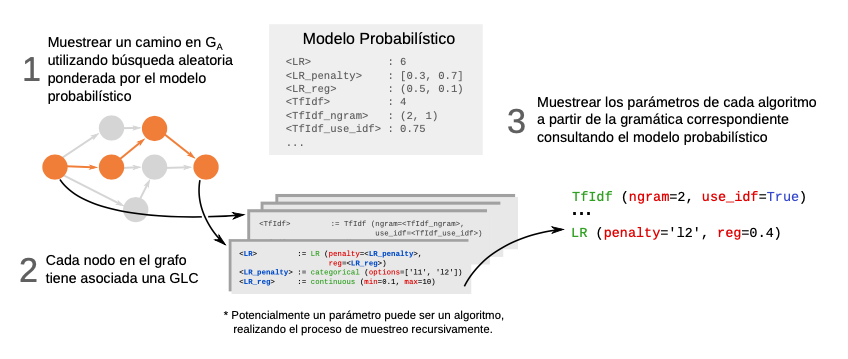
\includegraphics[scale=.5]{Figures/autogoal.png}
	\caption{Representación visual del proceso de creación y muestreo del
		espacio de búsqueda.}
	\label{fig:autogoal}
\end{figure}

El modelo $\sigma$ se inicializa con valores neutrales para cada distribución (pesos uniformes para distribución categórica, media centrada y máxima varianza para distribuciones continuas). El proceso de optimización consiste en un ciclo de generación y evaluación. Primeramente, se generan \texttt{n} flujos siguiendo el modelo de muestreo. Utilizando una función de evaluación $\Phi(p)$ (dada por el usuario para el problema a resolver) se evalúan los flujos y se seleccionan los $k < n$ mejores. El valor del mejor flujo del ciclo es comparado con el mejor global y actualizado en consecuencia. Tomando los valores de muestra de los hiperparámetros generados, se construye un modelo probabilístico marginal $\sigma^*$. Luego, el modelo $\sigma^*$ y el modelo marginal $\sigma$ son mezclados utilizando un factor de interpolación $\alpha \in [0, 1]$, ofreciendo un balance entre exploración y explotación. Este ciclo se repite hasta que se llegue a un límite de tiempo de ejecución, una cantidad determinada de iteraciones, o hasta que no se encuentre mejora. Por cada iteración el modelo $\sigma$ converge lentamente a un modelo que maximiza la probabilidad de producir los mejores flujos. 

La estrategia seguida para la inicialización del proceso de optimización de AutoGOAL es la modificación del modelo probabilístico $\sigma$. Después de obtener la lista de flujos de algoritmos recomendados en la fase de meta-learning, se extraen los modelos probabilísticos asociados a estos flujos. Estos modelos son guardados en la fase inicial de meta-learning, de obtención de meta-conocimiento, cuando se generan los flujos con AutoGOAL. Luego, se crea un modelo inicial $\sigma^*$, que es el resultado de la mezcla de los modelos probabilísticos de los flujos recomendados. En las primeras iteraciones se usa el modelo $\sigma$ con valores neutrales para cada distribución, generando flujos aleatorios, para lograr una mayor exploración y luego este modelo es mezclado con el modelo $\sigma^*$, que contiene las inicializaciones que son resultado de la fase de meta-learning. Al igual que en el proceso de optimización de AutoGOAL tradicional, se utiliza un factor de interpolación $\alpha \in [0, 1]$, ofreciendo un balance entre exploración y explotación. El resto del proceso de optimización de AutoGOAL ocurre normalmente.

